\section{Frontend System Design}
The frontend of the DBaaS platform is designed using a layered architecture to ensure scalability, maintainability, and a responsive user experience. It follows the \textbf{Model-View-ViewModel (MVVM)} pattern, which separates the graphical user interface from the underlying business logic.

Figure \ref{fig:frontend_arch} illustrates the internal structure of the Flutter application and how data flows between the different layers.

\begin{figure}[h]
    \centering
    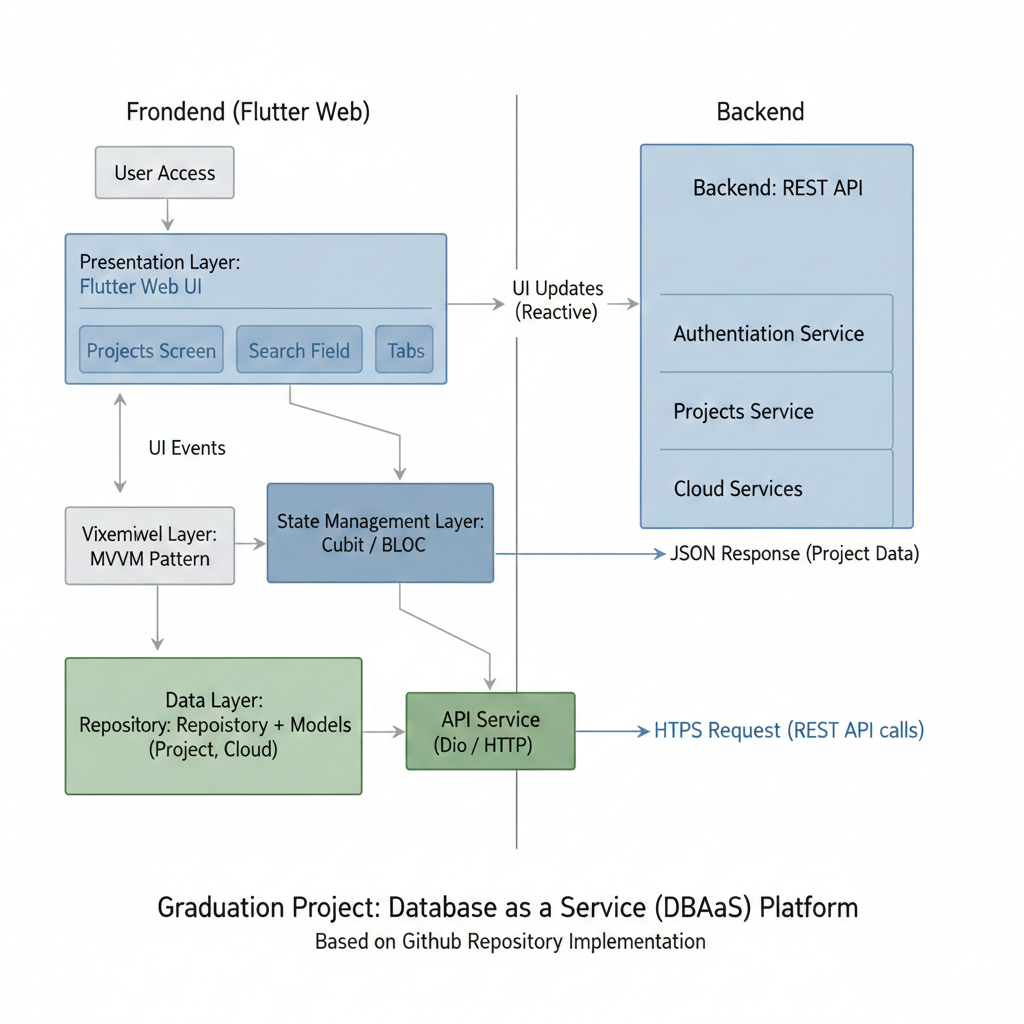
\includegraphics[width=0.9\textwidth]{images/UI/FE_arch.png}
    \caption{Frontend Layered Architecture (MVVM + BLoC)}
    \label{fig:frontend_arch}
\end{figure}

\subsection{Frontend Architectural Layers}
The architecture is structured into three primary layers as shown in the diagram:
\begin{itemize}
    \item \textbf{Presentation Layer:} Responsible for the Flutter Widgets and UI components that the user interacts with, ensuring a consistent and responsive experience across the platform.
    \item \textbf{State Management Layer (BLoC/Cubit):} Decouples the UI from business logic, managing project data and UI states effectively.
    \item \textbf{Data Layer:} Implements the Repository pattern to manage API services (Dio/HTTP), facilitating secure communication with the backend.
\end{itemize}

\subsection{Frontend Component Design}
To achieve a robust user experience, the frontend implements specialized components for data visualization and management:
\begin{itemize}
    \item \textbf{Schema Visualization Engine:} The system integrates a dynamic renderer for \textit{Mermaid.js}. This allows for the real-time conversion of AI-suggested schema JSON data into interactive, visual ERD diagrams within the browser, facilitating immediate architectural review.
    \item \textbf{High-Performance Data Tables:} The UI employs a virtualized table implementation to render database records. This approach ensures that even with large datasets, the UI remains responsive by rendering only the visible subset of data (server-side pagination).
    \item \textbf{Reactive Telemetry Dashboard:} The dashboard utilizes stream-based charting components. By decoupling telemetry data fetching from UI rendering, the system provides real-time performance insights without blocking the main event loop.
\end{itemize}
\subsection{Frontend Interaction & Data Flow}
The interaction model is designed to ensure both security and responsiveness:
\begin{itemize}
  \item \textbf{Authentication Flow:} Every interaction with the backend is guarded by an authentication layer. JWT tokens are securely stored and injected into the \textit{Authorization} header of every \texttt{http} request, ensuring all API calls are authenticated automatically and consistently.
    \item \textbf{Error Handling and Feedback:} The system implements a centralized error handling mechanism. All API failures (e.g., timeouts, unauthorized access, or 500 errors) are intercepted, logged, and translated into user-friendly notifications, preventing application crashes.
    \item \textbf{Asynchronous State Updates:} Given the nature of DBaaS operations (like schema generation or table creation), the UI utilizes asynchronous patterns. Users receive immediate feedback through progress indicators while the backend processes the request in the background, keeping the interface fluid.
\end{itemize}